\documentclass{article}

\usepackage{graphicx}
\usepackage{rotating}
\usepackage{amsmath}
\usepackage{fancyhdr}
\usepackage{listings}
\usepackage{xcolor}
\usepackage{color}
\usepackage{textcomp}
\usepackage{float}
\usepackage[sorting=none]{biblatex}
\usepackage[margin=1in]{geometry}
\usepackage[font={small,it}]{caption}
\usepackage{placeins}
\usepackage{xepersian}

%\DeclareMathOperator*{\btie}{\bowtie}
\addbibresource{bibliography.bib}
\settextfont[Scale=1.2]{B-NAZANIN.TTF}
\setlatintextfont[Scale=1]{Times New Roman}
\renewcommand{\baselinestretch}{1.5}
\pagestyle{fancy}
\fancyhf{}
\rhead{تکلیف اول درس مبانی بینایی کامپیوتر}
\lhead{\thepage}
\rfoot{علیرضا ابره فروش}
\lfoot{9816603}
\renewcommand{\headrulewidth}{1pt}
\renewcommand{\footrulewidth}{1pt}
%%%%%%%%%%
\lstset
{
    language=[latex]tex,
    basicstyle=\ttfamily,
    commentstyle=\color{black},
    columns=fullflexible,
    keepspaces=true,
    upquote=true,
    showstringspaces=false,
    morestring=[s]\\\%,
    stringstyle=\color{black},
}
%%%%%%%%%%
%beginMatlab
\definecolor{mygreen}{RGB}{28,172,0} % color values Red, Green, Blue
\definecolor{mylilas}{RGB}{170,55,241}
%endMatlab
\begin{document}
%beginMatlab
\lstset{language=Matlab,%
    %basicstyle=\color{red},
    breaklines=true,%
    morekeywords={matlab2tikz},
    keywordstyle=\color{blue},%
    morekeywords=[2]{1}, keywordstyle=[2]{\color{black}},
    identifierstyle=\color{black},%
    stringstyle=\color{mylilas},
    commentstyle=\color{mygreen},%
    showstringspaces=false,%without this there will be a symbol in the places where there is a space
    numbers=left,%
    numberstyle={\tiny \color{black}},% size of the numbers
    numbersep=9pt, % this defines how far the numbers are from the text
    emph=[1]{for,end,break},emphstyle=[1]\color{red}, %some words to emphasise
    %emph=[2]{word1,word2}, emphstyle=[2]{style},    
}
%endMatlab
\begin{titlepage}
\begin{center}

\includegraphics[width=0.4\textwidth]{figures/IUT Logo.png}\\
        
\LARGE
\textbf{دانشگاه صنعتی اصفهان}\\
\textbf{دانشکده مهندسی برق و کامپیوتر}\\
        
\vfill
        
\huge
\textbf{عنوان: تکلیف چهارم درس ریزپردازنده}\\
        
\vfill
        
\LARGE
\textbf{نام و نام خانوادگی: علیرضا ابره فروش}\\
\textbf{شماره دانشجویی: 9816603}\\
\textbf{نیم\,سال تحصیلی: پاییز 1400}\\
\textbf{مدرّس: دکتر عارف کریمی افشار}\\
\end{center}
\end{titlepage}


%\tableofcontents
\newpage


\section{}%1
ابتدا فایل تصویر را با نرم‌افزار \lr{Notepad} باز می‌کنیم. با توجه به شکل زیر، ابعاد تصویر
852
$\times$
1282 است و همچنین ماکسیممِ سطح روشناییِ هر کانال رنگیِ هر پیکسل 255 است. در نهایت می‌توان حدس زد که دیتای تصویر از کاراکتر هفدهم به بعد باشد.
\begin{figure}[H]
    \centering
    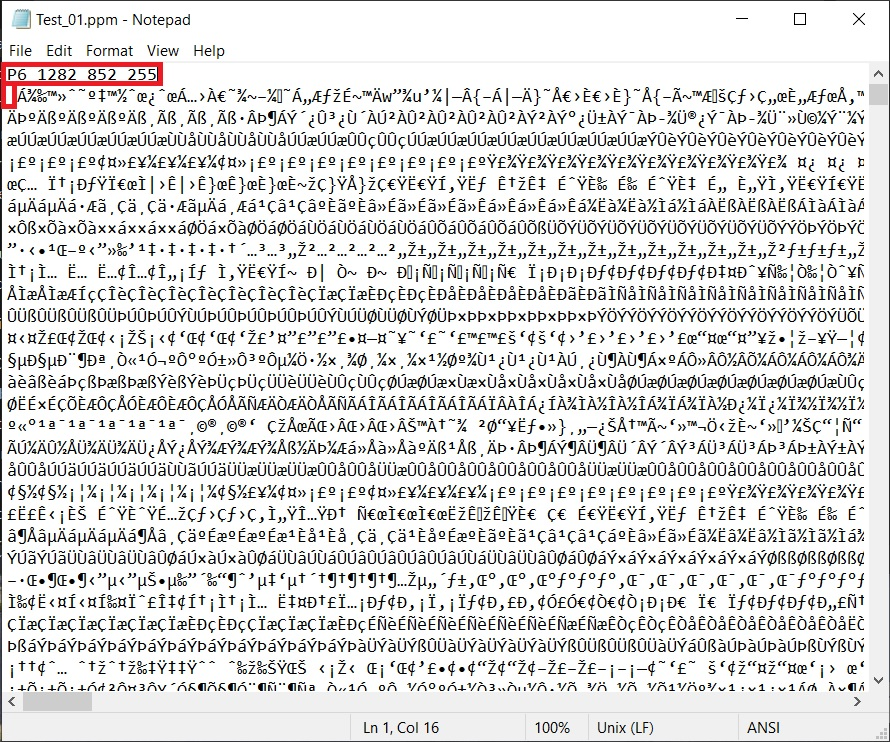
\includegraphics[width=1\textwidth]{figures/1a.jpg}
    \caption
	{
تصویر
	}
    \label{fig:fig1}
\end{figure}
حال تصویر را هم با دستور \lr{fopen} و \lr{fread} و هم با استفاده از دستور \lr{imtool} باز می‌کنیم. اگر به تصاویر زیر دقت کنیم می‌بینیم که حدس ما برای اولین کاراکتر دیتای تصویر درست است و سطح روشنایی اولین پیکسل تصویر در بایت هفدهم این فایل قرار دارد. همچنین با مشاهده خروجی دستور \lr{imtool} و مقایسه با آرایه‌ی نظیر فایل می‌بینیم که سطح روشنایی نظیر رنگ‌های قرمز، سبز و آبی به ترتیب در اندیس‌های مضرب 3 به علاوه‌ی 2، مضرب 3 و مضرب 3 به علاوه‌ی 1 ذخیره شده‌اند.
\begin{figure}[H]
    \centering
    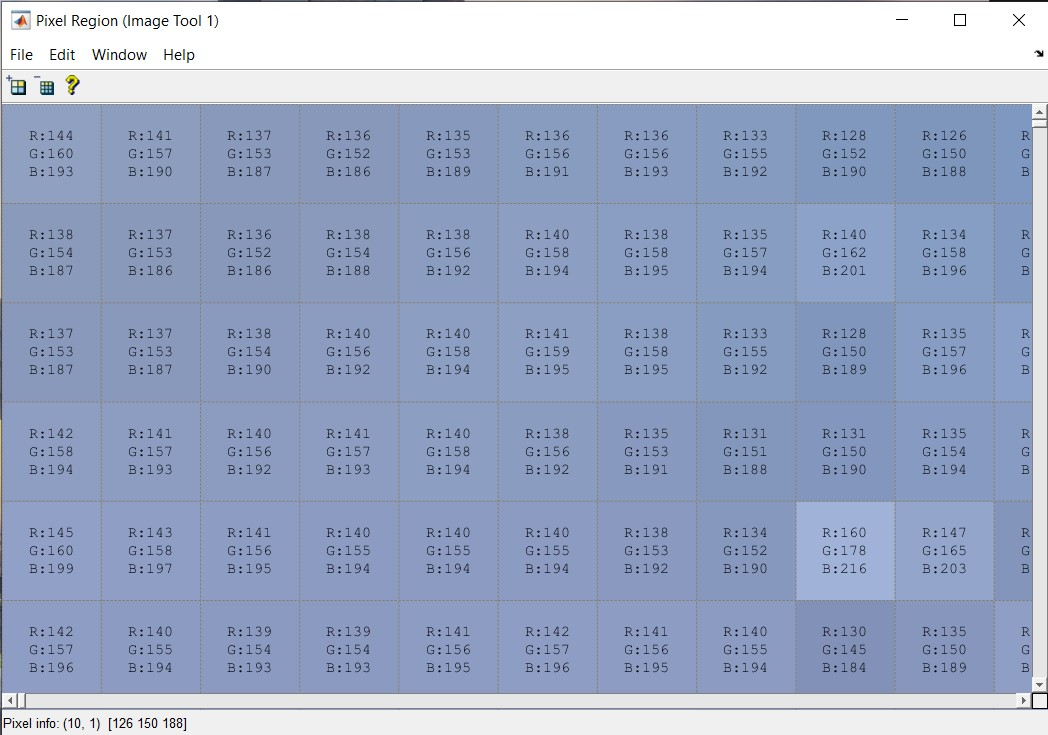
\includegraphics[width=0.8\textwidth]{figures/1b.jpg}
    \caption
	{
تصویر
	}
    \label{fig:fig1}
\end{figure}
\begin{figure}[H]
    \centering
    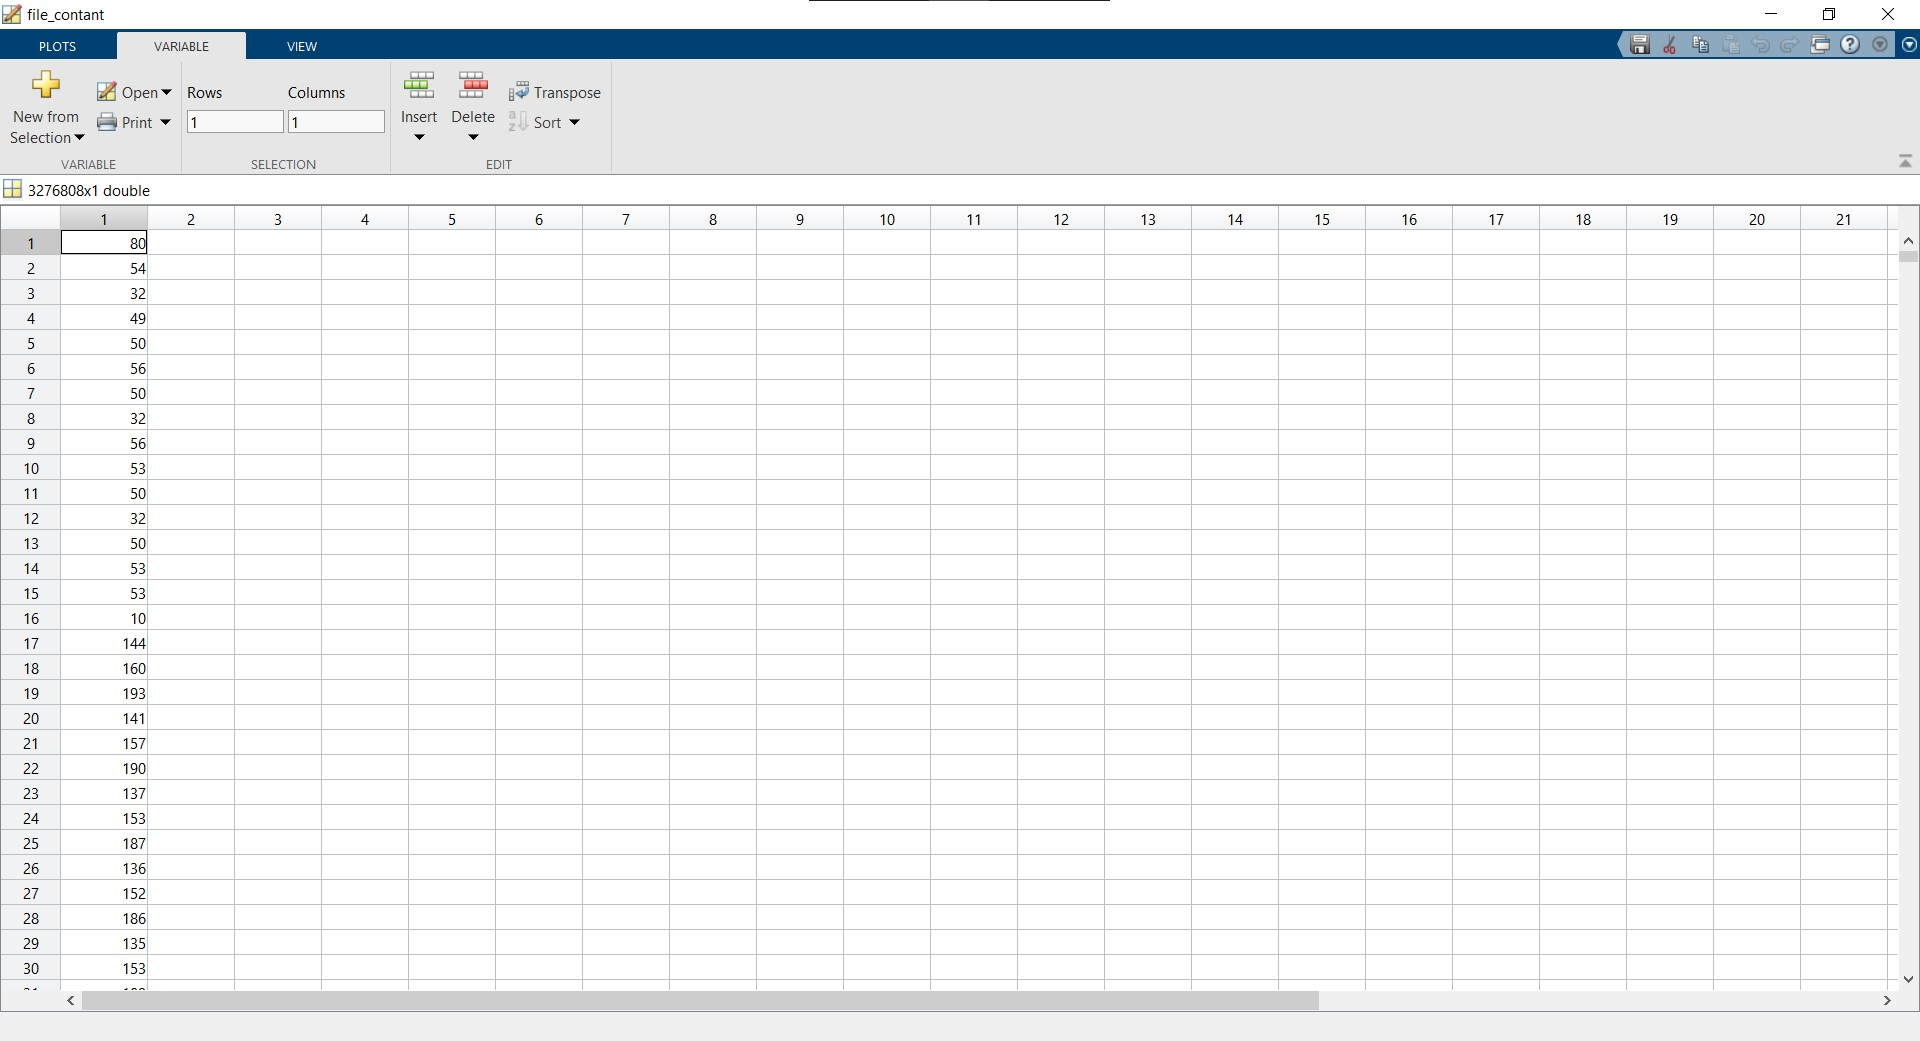
\includegraphics[width=0.8\textwidth]{figures/1c.jpg}
    \caption
	{
تصویر
	}
    \label{fig:fig1}
\end{figure}
پس برای خواندن تصویر ورودی در محیط برنامه‌نویسی مورد نظر و دسترسی به داده‌های آن به شکل زیر عمل می‌کنیم.
\begin{latin}
\lstinputlisting{sources/p1.m}
\end{latin}
و در آخر می‌بینیم که خروجی‌ها یکسان هستند.
\begin{figure}[H]
    \centering
    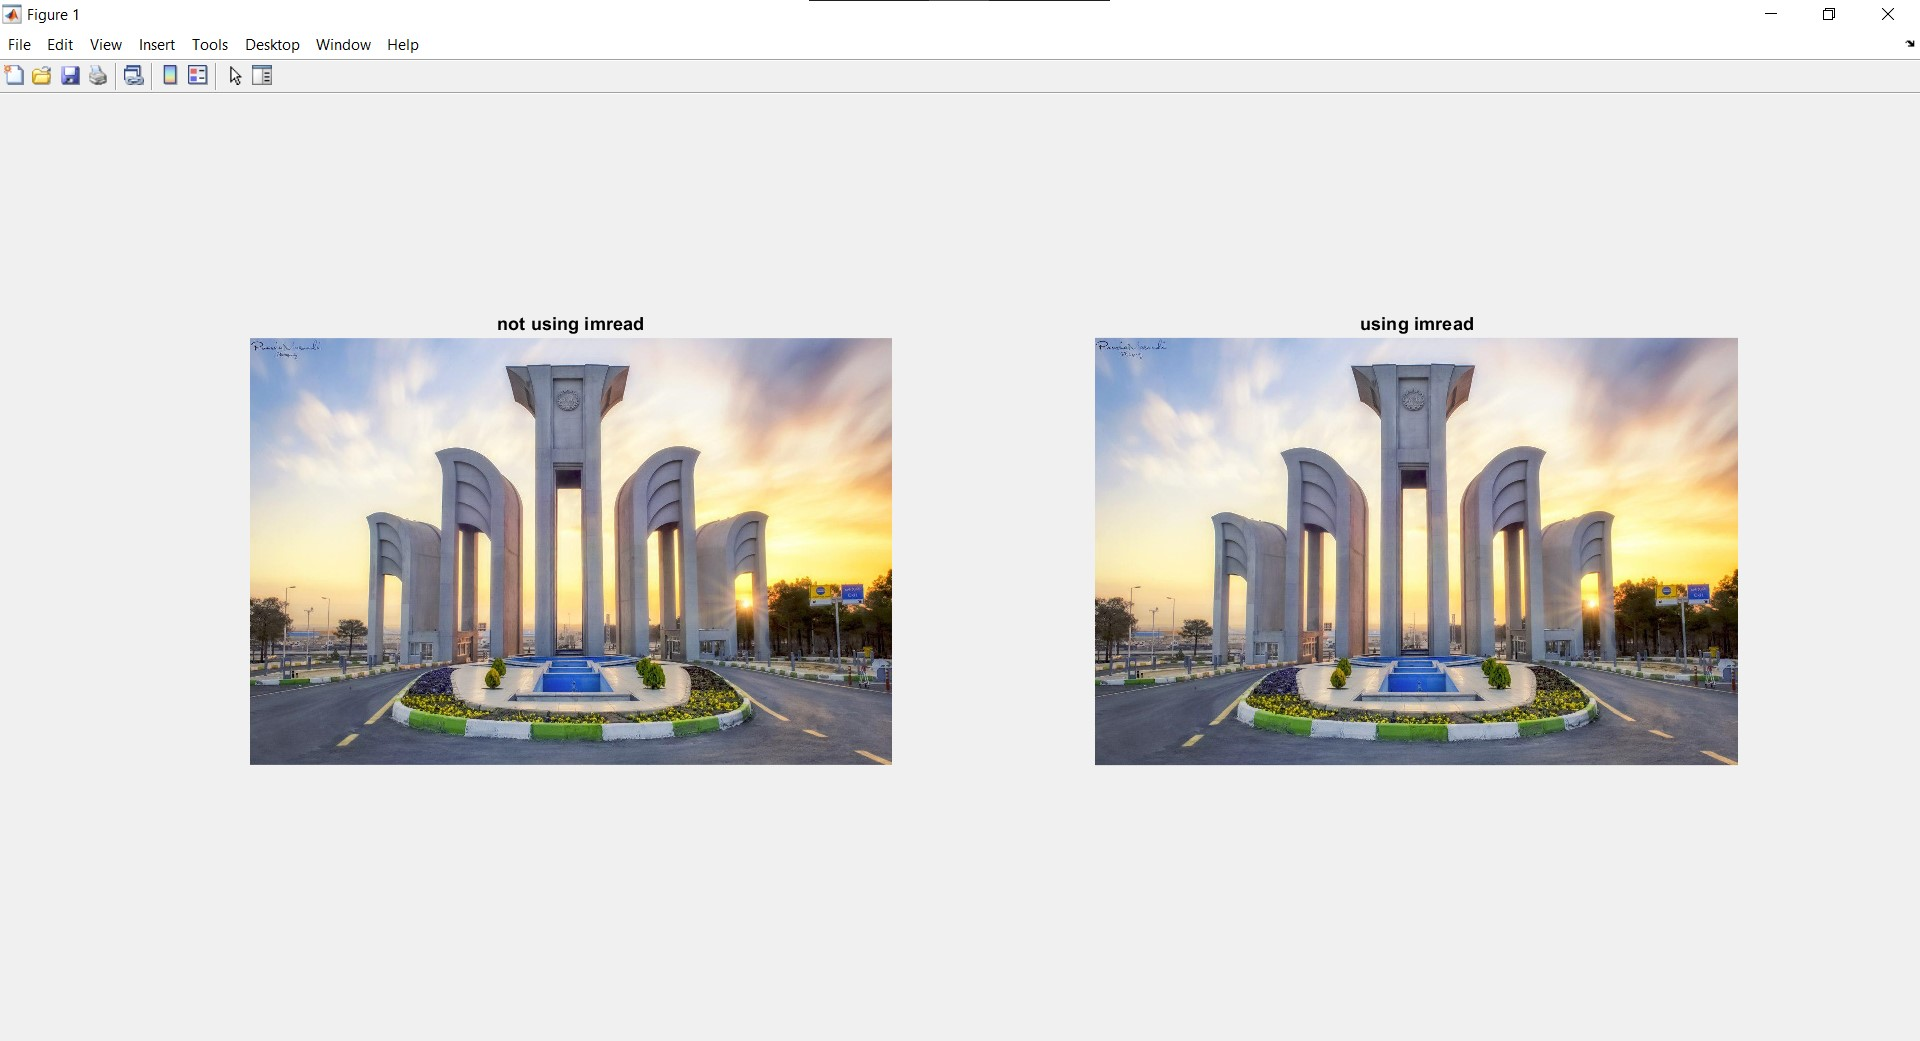
\includegraphics[width=1\textwidth]{figures/1d.jpg}
    \caption
	{
تصویر خروجی سوال 1
	}
    \label{fig:fig1}
\end{figure}


\section{}%2
برای این کار می‌توان ابتدا تصویر را \lr{Grayscale} کرد، سپس ناحیه‌ی بیضی شکل را قرمز کرد و در نهایت ناحیه لوزی شکل را با مقادیر اولیه‌ی تصویر مقداردهی کرد.
\begin{latin}
\lstinputlisting{sources/p2.m}
\end{latin}

\begin{figure}[H]
    \centering
    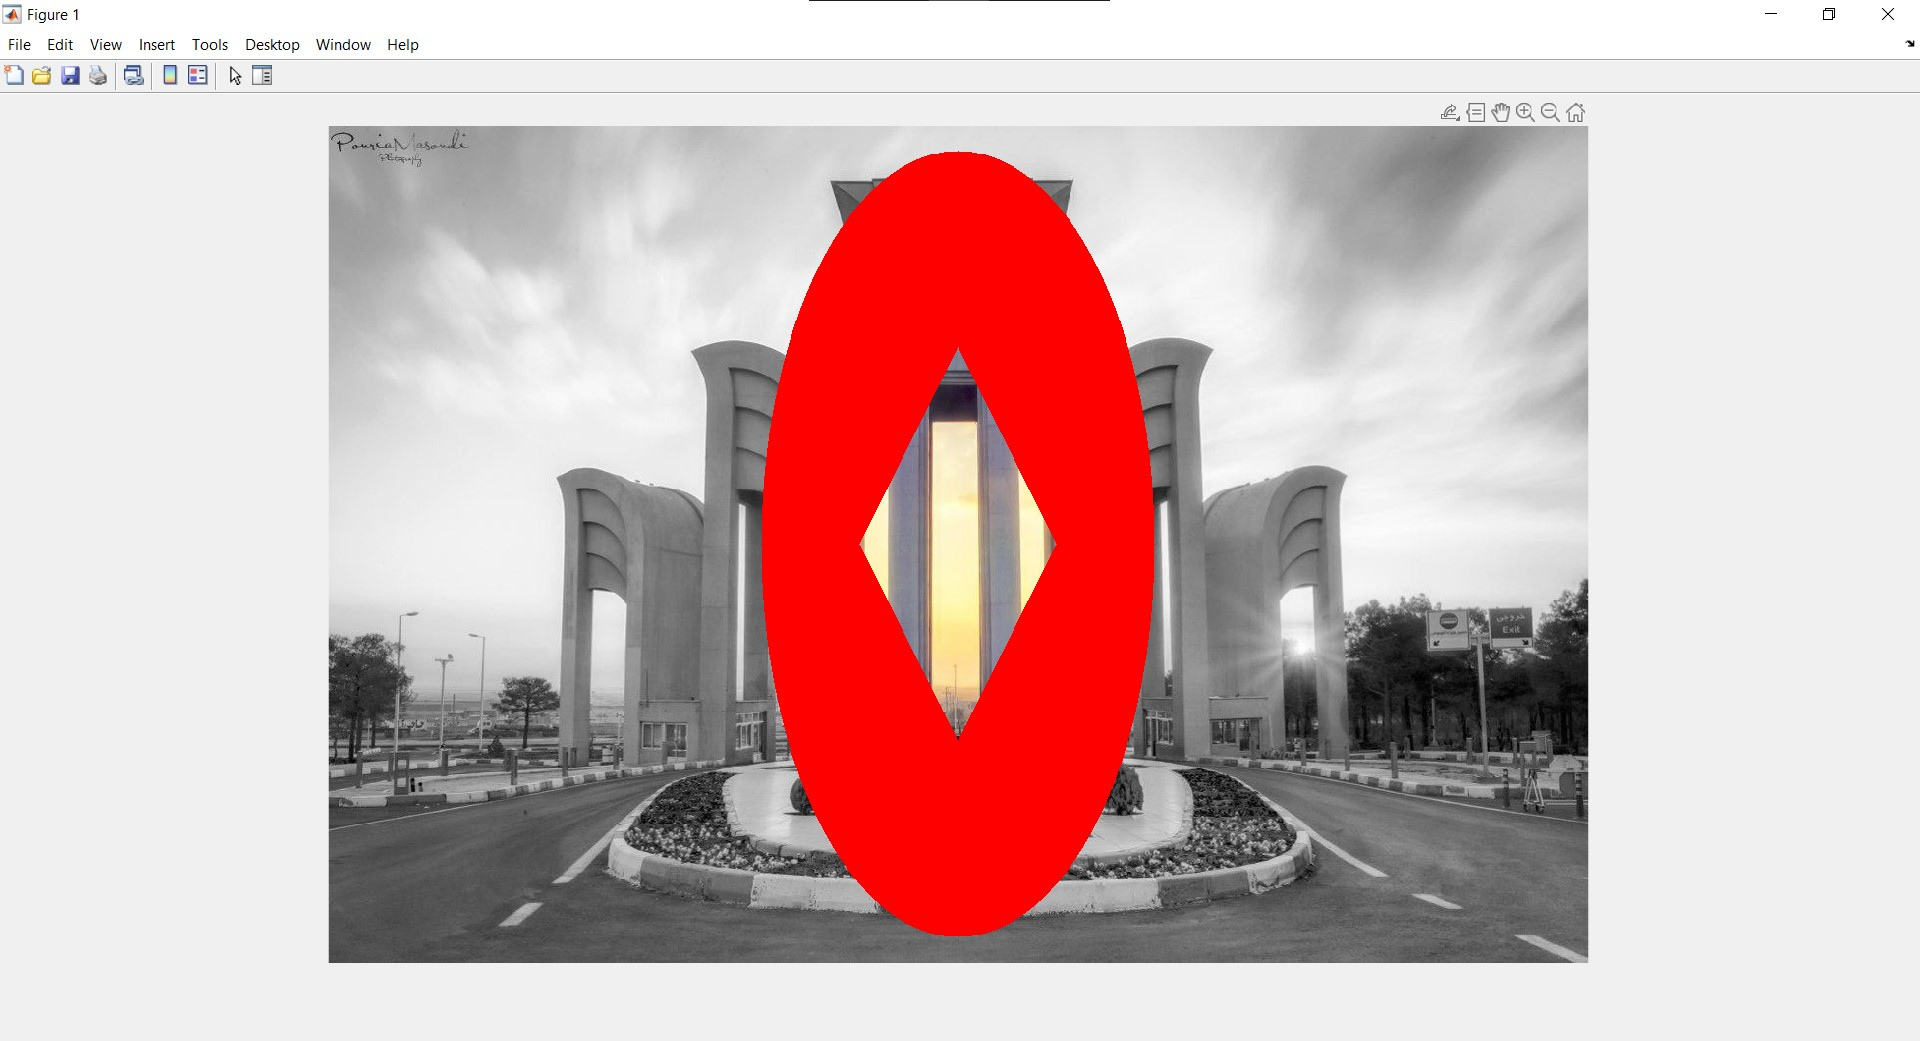
\includegraphics[width=1\textwidth]{figures/2a.jpg}
    \caption
	{
تصویر خروجی سوال 2
	}
    \label{fig:fig1}
\end{figure}


\section{}%3
ابتدا با استفاده از روابط زیر طول و عرض جدید تصویر را محاسبه می‌کنیم:
\newline
$
h_{new} = \left\lceil \left| w \times sin(\theta) \right| + \left| h \times cos(\theta) \right| \right\rceil
\newline
w_{new} = \left\lceil \left| h \times sin(\theta) \right| + \left| w \times cos(\theta) \right| \right\rceil
\newline
$
سپس با استفاده از روابط ماتریس دوران، مختصات پیکسلِ نظیرِ پیکسلِ دوران یافته را پیدا می‌کنیم و مقادیر \lr{RGB}اش را برابر آن پیکسل قرار می‌دهیم. تابع \lr{rotateImage} این کار را انجام می‌دهد.


\begin{latin}
\lstinputlisting{sources/rotateImage.m}
\end{latin}
در نهایت تابع را به ازای زاویه‌ی 60 درجه فراخوانی می‌کنیم.
\begin{latin}
\lstinputlisting{sources/p3.m}
\end{latin}

\begin{figure}[H]
    \centering
    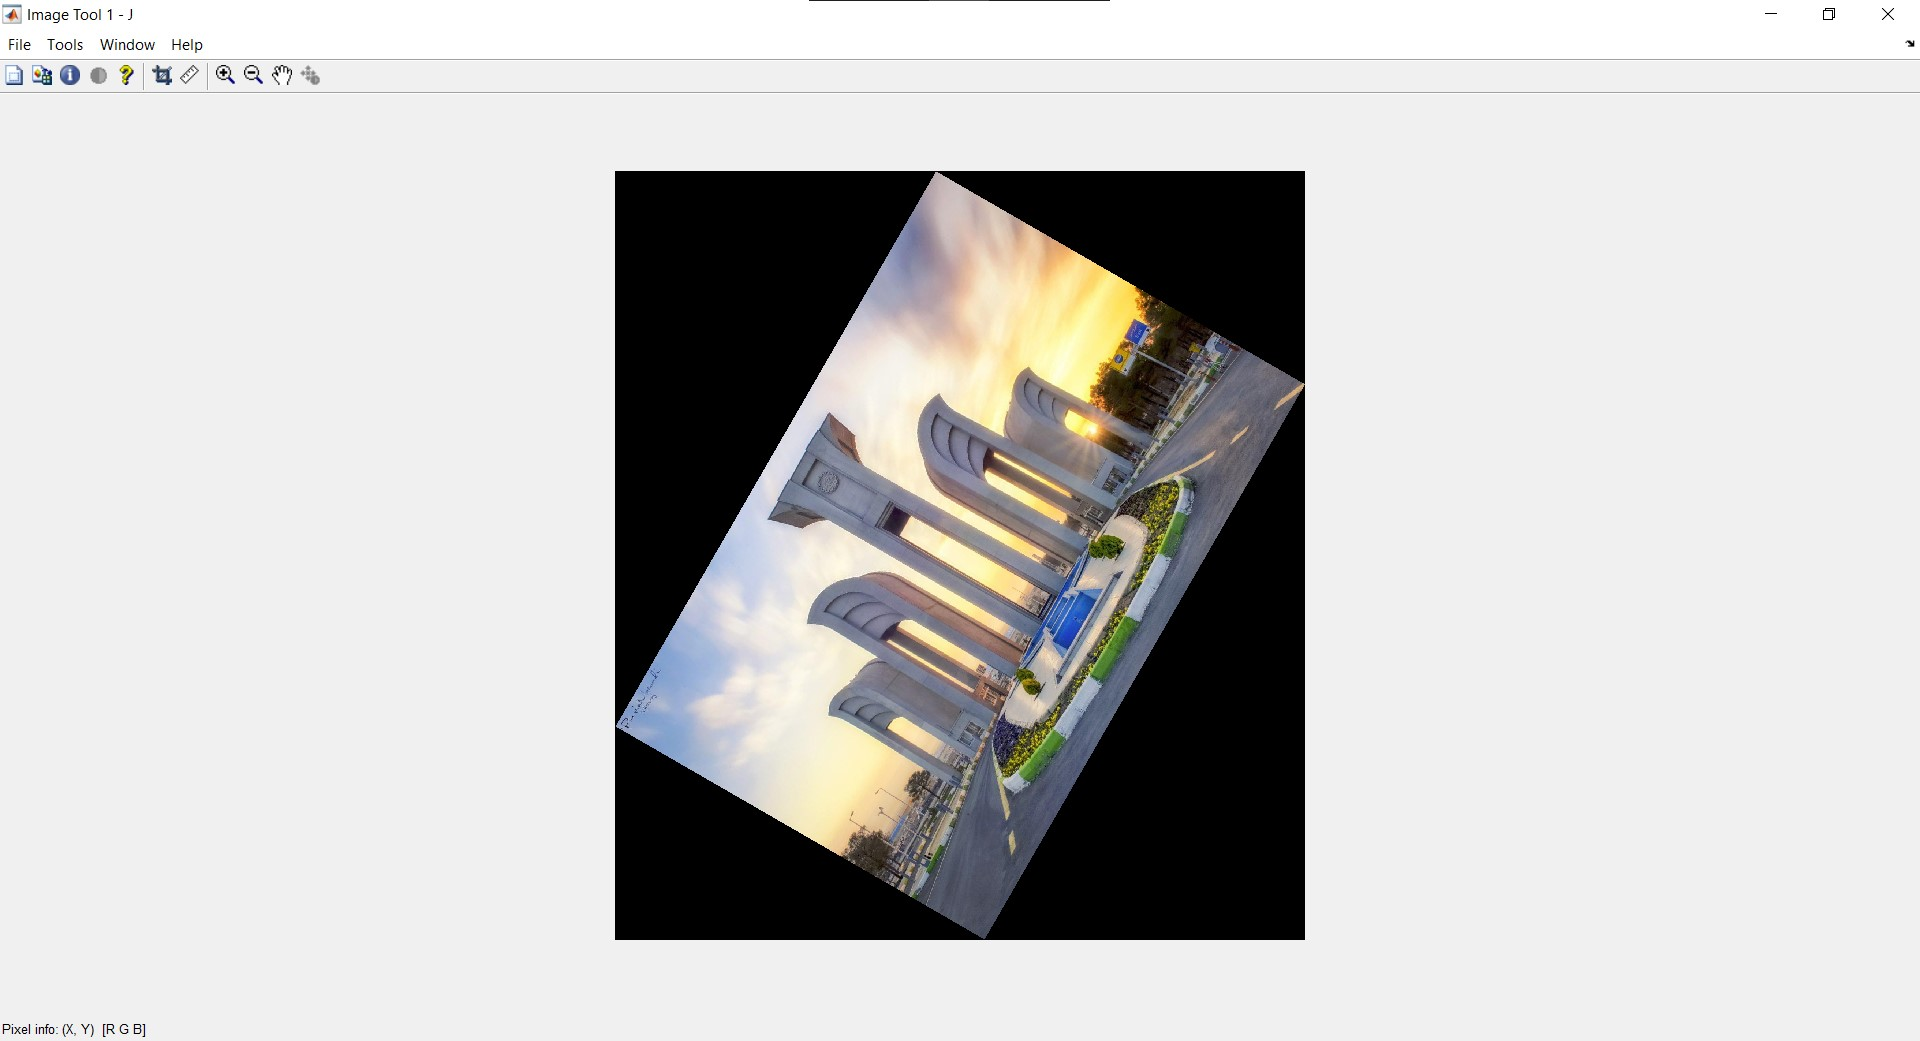
\includegraphics[width=1\textwidth]{figures/3a.jpg}
    \caption
	{
نمونه تصویر خروجی سوال 3 برای زاویه‌ی 60 درجه
	}
    \label{fig:fig1}
\end{figure}
%%%%%%%%%%%%%%%%%%%%%%%%%%%%%%%%%%%
%%%%%%%%%%%%%%%%%%%%%%%%%%%%%%%%%%%
%%%%%%%%%%%%%%%%%%%%%%%%%%%%%%%%%%%

%------------------------------------------------------------------------------------------


\section*{منابع}
\renewcommand{\section}[2]{}%
\begin{thebibliography}{99} % assumes less than 100 references
%چنانچه مرجع فارسی نیز داشته باشید باید دستور فوق را فعال کنید و مراجع فارسی خود را بعد از این دستور وارد کنید


\begin{LTRitems}

\resetlatinfont

\bibitem{b1}
\end{LTRitems}

\end{thebibliography}


\end{document}
